% Created by tikzDevice version 0.12.3.1 on 2023-05-29 17:50:57
% !TEX encoding = UTF-8 Unicode
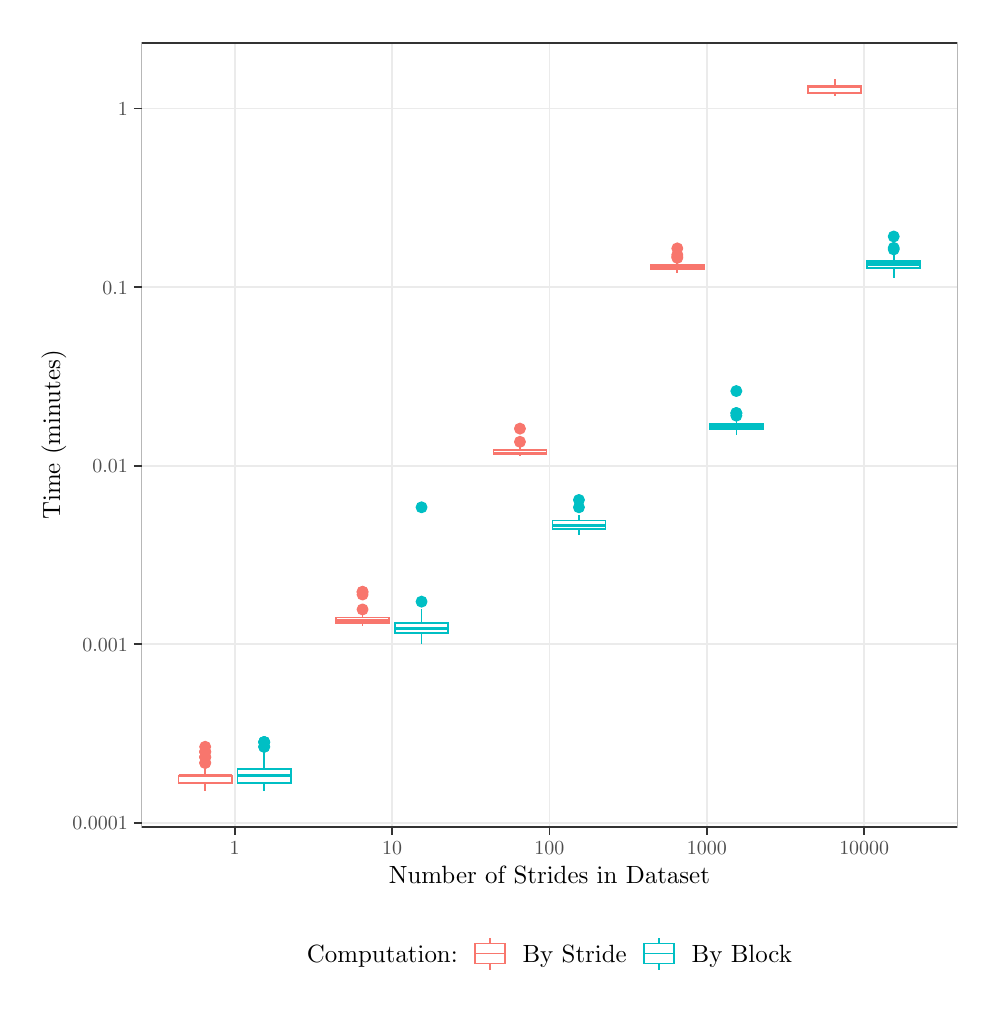
\begin{tikzpicture}[x=1pt,y=1pt]
\definecolor{fillColor}{RGB}{255,255,255}
\path[use as bounding box,fill=fillColor,fill opacity=0.00] (0,0) rectangle (341.43,352.81);
\begin{scope}
\path[clip] (  0.00,  0.00) rectangle (341.43,352.81);
\definecolor{drawColor}{RGB}{255,255,255}
\definecolor{fillColor}{RGB}{255,255,255}

\path[draw=drawColor,line width= 0.6pt,line join=round,line cap=round,fill=fillColor] (  0.00,  0.00) rectangle (341.43,352.81);
\end{scope}
\begin{scope}
\path[clip] ( 41.14, 63.96) rectangle (335.93,347.31);
\definecolor{fillColor}{RGB}{255,255,255}

\path[fill=fillColor] ( 41.14, 63.96) rectangle (335.93,347.31);
\definecolor{drawColor}{gray}{0.92}

\path[draw=drawColor,line width= 0.6pt,line join=round] ( 41.14, 65.48) --
	(335.93, 65.48);

\path[draw=drawColor,line width= 0.6pt,line join=round] ( 41.14,130.00) --
	(335.93,130.00);

\path[draw=drawColor,line width= 0.6pt,line join=round] ( 41.14,194.51) --
	(335.93,194.51);

\path[draw=drawColor,line width= 0.6pt,line join=round] ( 41.14,259.03) --
	(335.93,259.03);

\path[draw=drawColor,line width= 0.6pt,line join=round] ( 41.14,323.55) --
	(335.93,323.55);

\path[draw=drawColor,line width= 0.6pt,line join=round] ( 74.80, 63.96) --
	( 74.80,347.31);

\path[draw=drawColor,line width= 0.6pt,line join=round] (131.67, 63.96) --
	(131.67,347.31);

\path[draw=drawColor,line width= 0.6pt,line join=round] (188.54, 63.96) --
	(188.54,347.31);

\path[draw=drawColor,line width= 0.6pt,line join=round] (245.41, 63.96) --
	(245.41,347.31);

\path[draw=drawColor,line width= 0.6pt,line join=round] (302.27, 63.96) --
	(302.27,347.31);
\definecolor{drawColor}{RGB}{248,118,109}
\definecolor{fillColor}{RGB}{248,118,109}

\path[draw=drawColor,line width= 0.4pt,line join=round,line cap=round,fill=fillColor] ( 64.14, 89.22) circle (  1.96);

\path[draw=drawColor,line width= 0.4pt,line join=round,line cap=round,fill=fillColor] ( 64.14, 89.22) circle (  1.96);

\path[draw=drawColor,line width= 0.4pt,line join=round,line cap=round,fill=fillColor] ( 64.14, 87.14) circle (  1.96);

\path[draw=drawColor,line width= 0.4pt,line join=round,line cap=round,fill=fillColor] ( 64.14, 91.15) circle (  1.96);

\path[draw=drawColor,line width= 0.4pt,line join=round,line cap=round,fill=fillColor] ( 64.14, 92.96) circle (  1.96);

\path[draw=drawColor,line width= 0.4pt,line join=round,line cap=round,fill=fillColor] ( 64.14, 91.15) circle (  1.96);

\path[draw=drawColor,line width= 0.4pt,line join=round,line cap=round,fill=fillColor] ( 64.14, 91.15) circle (  1.96);

\path[draw=drawColor,line width= 0.4pt,line join=round,line cap=round,fill=fillColor] ( 64.14, 87.14) circle (  1.96);

\path[draw=drawColor,line width= 0.4pt,line join=round,line cap=round,fill=fillColor] ( 64.14, 89.22) circle (  1.96);

\path[draw=drawColor,line width= 0.6pt,line join=round] ( 64.14, 82.46) -- ( 64.14, 84.90);

\path[draw=drawColor,line width= 0.6pt,line join=round] ( 64.14, 79.79) -- ( 64.14, 76.84);
\definecolor{fillColor}{RGB}{255,255,255}

\path[draw=drawColor,line width= 0.6pt,fill=fillColor] ( 54.54, 82.46) --
	( 54.54, 79.79) --
	( 73.74, 79.79) --
	( 73.74, 82.46) --
	( 54.54, 82.46) --
	cycle;

\path[draw=drawColor,line width= 1.1pt] ( 54.54, 82.46) -- ( 73.74, 82.46);
\definecolor{fillColor}{RGB}{248,118,109}

\path[draw=drawColor,line width= 0.4pt,line join=round,line cap=round,fill=fillColor] (121.01,148.95) circle (  1.96);

\path[draw=drawColor,line width= 0.4pt,line join=round,line cap=round,fill=fillColor] (121.01,148.95) circle (  1.96);

\path[draw=drawColor,line width= 0.4pt,line join=round,line cap=round,fill=fillColor] (121.01,142.58) circle (  1.96);

\path[draw=drawColor,line width= 0.4pt,line join=round,line cap=round,fill=fillColor] (121.01,147.98) circle (  1.96);

\path[draw=drawColor,line width= 0.6pt,line join=round] (121.01,139.67) -- (121.01,141.04);

\path[draw=drawColor,line width= 0.6pt,line join=round] (121.01,137.79) -- (121.01,136.62);
\definecolor{fillColor}{RGB}{255,255,255}

\path[draw=drawColor,line width= 0.6pt,fill=fillColor] (111.41,139.67) --
	(111.41,137.79) --
	(130.60,137.79) --
	(130.60,139.67) --
	(111.41,139.67) --
	cycle;

\path[draw=drawColor,line width= 1.1pt] (111.41,138.75) -- (130.60,138.75);
\definecolor{fillColor}{RGB}{248,118,109}

\path[draw=drawColor,line width= 0.4pt,line join=round,line cap=round,fill=fillColor] (177.88,203.16) circle (  1.96);

\path[draw=drawColor,line width= 0.4pt,line join=round,line cap=round,fill=fillColor] (177.88,207.92) circle (  1.96);

\path[draw=drawColor,line width= 0.6pt,line join=round] (177.88,200.15) -- (177.88,202.15);

\path[draw=drawColor,line width= 0.6pt,line join=round] (177.88,198.56) -- (177.88,198.02);
\definecolor{fillColor}{RGB}{255,255,255}

\path[draw=drawColor,line width= 0.6pt,fill=fillColor] (168.28,200.15) --
	(168.28,198.56) --
	(187.47,198.56) --
	(187.47,200.15) --
	(168.28,200.15) --
	cycle;

\path[draw=drawColor,line width= 1.1pt] (168.28,199.07) -- (187.47,199.07);
\definecolor{fillColor}{RGB}{248,118,109}

\path[draw=drawColor,line width= 0.4pt,line join=round,line cap=round,fill=fillColor] (234.74,270.03) circle (  1.96);

\path[draw=drawColor,line width= 0.4pt,line join=round,line cap=round,fill=fillColor] (234.74,273.05) circle (  1.96);

\path[draw=drawColor,line width= 0.4pt,line join=round,line cap=round,fill=fillColor] (234.74,269.64) circle (  1.96);

\path[draw=drawColor,line width= 0.4pt,line join=round,line cap=round,fill=fillColor] (234.74,270.76) circle (  1.96);

\path[draw=drawColor,line width= 0.6pt,line join=round] (234.74,267.06) -- (234.74,269.53);

\path[draw=drawColor,line width= 0.6pt,line join=round] (234.74,265.38) -- (234.74,264.31);
\definecolor{fillColor}{RGB}{255,255,255}

\path[draw=drawColor,line width= 0.6pt,fill=fillColor] (225.15,267.06) --
	(225.15,265.38) --
	(244.34,265.38) --
	(244.34,267.06) --
	(225.15,267.06) --
	cycle;

\path[draw=drawColor,line width= 1.1pt] (225.15,266.18) -- (244.34,266.18);

\path[draw=drawColor,line width= 0.6pt,line join=round] (291.61,331.91) -- (291.61,334.43);

\path[draw=drawColor,line width= 0.6pt,line join=round] (291.61,329.18) -- (291.61,328.10);

\path[draw=drawColor,line width= 0.6pt,fill=fillColor] (282.01,331.91) --
	(282.01,329.18) --
	(301.21,329.18) --
	(301.21,331.91) --
	(282.01,331.91) --
	cycle;

\path[draw=drawColor,line width= 1.1pt] (282.01,331.63) -- (301.21,331.63);
\definecolor{drawColor}{RGB}{0,191,196}
\definecolor{fillColor}{RGB}{0,191,196}

\path[draw=drawColor,line width= 0.4pt,line join=round,line cap=round,fill=fillColor] ( 85.46, 94.66) circle (  1.96);

\path[draw=drawColor,line width= 0.4pt,line join=round,line cap=round,fill=fillColor] ( 85.46, 92.96) circle (  1.96);

\path[draw=drawColor,line width= 0.4pt,line join=round,line cap=round,fill=fillColor] ( 85.46, 94.66) circle (  1.96);

\path[draw=drawColor,line width= 0.4pt,line join=round,line cap=round,fill=fillColor] ( 85.46, 92.96) circle (  1.96);

\path[draw=drawColor,line width= 0.4pt,line join=round,line cap=round,fill=fillColor] ( 85.46, 94.66) circle (  1.96);

\path[draw=drawColor,line width= 0.6pt,line join=round] ( 85.46, 84.90) -- ( 85.46, 91.15);

\path[draw=drawColor,line width= 0.6pt,line join=round] ( 85.46, 79.79) -- ( 85.46, 76.84);
\definecolor{fillColor}{RGB}{255,255,255}

\path[draw=drawColor,line width= 0.6pt,fill=fillColor] ( 75.87, 84.90) --
	( 75.87, 79.79) --
	( 95.06, 79.79) --
	( 95.06, 84.90) --
	( 75.87, 84.90) --
	cycle;

\path[draw=drawColor,line width= 1.1pt] ( 75.87, 82.46) -- ( 95.06, 82.46);
\definecolor{fillColor}{RGB}{0,191,196}

\path[draw=drawColor,line width= 0.4pt,line join=round,line cap=round,fill=fillColor] (142.33,145.41) circle (  1.96);

\path[draw=drawColor,line width= 0.4pt,line join=round,line cap=round,fill=fillColor] (142.33,179.49) circle (  1.96);

\path[draw=drawColor,line width= 0.6pt,line join=round] (142.33,137.62) -- (142.33,142.58);

\path[draw=drawColor,line width= 0.6pt,line join=round] (142.33,134.01) -- (142.33,130.00);
\definecolor{fillColor}{RGB}{255,255,255}

\path[draw=drawColor,line width= 0.6pt,fill=fillColor] (132.74,137.62) --
	(132.74,134.01) --
	(151.93,134.01) --
	(151.93,137.62) --
	(132.74,137.62) --
	cycle;

\path[draw=drawColor,line width= 1.1pt] (132.74,135.87) -- (151.93,135.87);
\definecolor{fillColor}{RGB}{0,191,196}

\path[draw=drawColor,line width= 0.4pt,line join=round,line cap=round,fill=fillColor] (199.20,179.49) circle (  1.96);

\path[draw=drawColor,line width= 0.4pt,line join=round,line cap=round,fill=fillColor] (199.20,182.15) circle (  1.96);

\path[draw=drawColor,line width= 0.6pt,line join=round] (199.20,174.67) -- (199.20,176.81);

\path[draw=drawColor,line width= 0.6pt,line join=round] (199.20,171.62) -- (199.20,169.42);
\definecolor{fillColor}{RGB}{255,255,255}

\path[draw=drawColor,line width= 0.6pt,fill=fillColor] (189.60,174.67) --
	(189.60,171.62) --
	(208.80,171.62) --
	(208.80,174.67) --
	(189.60,174.67) --
	cycle;

\path[draw=drawColor,line width= 1.1pt] (189.60,172.96) -- (208.80,172.96);
\definecolor{fillColor}{RGB}{0,191,196}

\path[draw=drawColor,line width= 0.4pt,line join=round,line cap=round,fill=fillColor] (256.07,212.60) circle (  1.96);

\path[draw=drawColor,line width= 0.4pt,line join=round,line cap=round,fill=fillColor] (256.07,213.54) circle (  1.96);

\path[draw=drawColor,line width= 0.4pt,line join=round,line cap=round,fill=fillColor] (256.07,221.50) circle (  1.96);

\path[draw=drawColor,line width= 0.4pt,line join=round,line cap=round,fill=fillColor] (256.07,213.56) circle (  1.96);

\path[draw=drawColor,line width= 0.6pt,line join=round] (256.07,209.68) -- (256.07,211.75);

\path[draw=drawColor,line width= 0.6pt,line join=round] (256.07,207.75) -- (256.07,205.62);
\definecolor{fillColor}{RGB}{255,255,255}

\path[draw=drawColor,line width= 0.6pt,fill=fillColor] (246.47,209.68) --
	(246.47,207.75) --
	(265.66,207.75) --
	(265.66,209.68) --
	(246.47,209.68) --
	cycle;

\path[draw=drawColor,line width= 1.1pt] (246.47,208.81) -- (265.66,208.81);
\definecolor{fillColor}{RGB}{0,191,196}

\path[draw=drawColor,line width= 0.4pt,line join=round,line cap=round,fill=fillColor] (312.94,277.35) circle (  1.96);

\path[draw=drawColor,line width= 0.4pt,line join=round,line cap=round,fill=fillColor] (312.94,272.69) circle (  1.96);

\path[draw=drawColor,line width= 0.4pt,line join=round,line cap=round,fill=fillColor] (312.94,273.24) circle (  1.96);

\path[draw=drawColor,line width= 0.6pt,line join=round] (312.94,268.60) -- (312.94,272.20);

\path[draw=drawColor,line width= 0.6pt,line join=round] (312.94,266.07) -- (312.94,262.35);
\definecolor{fillColor}{RGB}{255,255,255}

\path[draw=drawColor,line width= 0.6pt,fill=fillColor] (303.34,268.60) --
	(303.34,266.07) --
	(322.53,266.07) --
	(322.53,268.60) --
	(303.34,268.60) --
	cycle;

\path[draw=drawColor,line width= 1.1pt] (303.34,267.41) -- (322.53,267.41);
\definecolor{drawColor}{gray}{0.20}

\path[draw=drawColor,line width= 0.6pt,line join=round,line cap=round] ( 41.14, 63.96) rectangle (335.93,347.31);
\end{scope}
\begin{scope}
\path[clip] (  0.00,  0.00) rectangle (341.43,352.81);
\definecolor{drawColor}{gray}{0.30}

\node[text=drawColor,anchor=base east,inner sep=0pt, outer sep=0pt, scale=  0.72] at ( 36.19, 63.00) {0.0001};

\node[text=drawColor,anchor=base east,inner sep=0pt, outer sep=0pt, scale=  0.72] at ( 36.19,127.52) {0.001};

\node[text=drawColor,anchor=base east,inner sep=0pt, outer sep=0pt, scale=  0.72] at ( 36.19,192.03) {0.01};

\node[text=drawColor,anchor=base east,inner sep=0pt, outer sep=0pt, scale=  0.72] at ( 36.19,256.55) {0.1};

\node[text=drawColor,anchor=base east,inner sep=0pt, outer sep=0pt, scale=  0.72] at ( 36.19,321.07) {1};
\end{scope}
\begin{scope}
\path[clip] (  0.00,  0.00) rectangle (341.43,352.81);
\definecolor{drawColor}{gray}{0.20}

\path[draw=drawColor,line width= 0.6pt,line join=round] ( 38.39, 65.48) --
	( 41.14, 65.48);

\path[draw=drawColor,line width= 0.6pt,line join=round] ( 38.39,130.00) --
	( 41.14,130.00);

\path[draw=drawColor,line width= 0.6pt,line join=round] ( 38.39,194.51) --
	( 41.14,194.51);

\path[draw=drawColor,line width= 0.6pt,line join=round] ( 38.39,259.03) --
	( 41.14,259.03);

\path[draw=drawColor,line width= 0.6pt,line join=round] ( 38.39,323.55) --
	( 41.14,323.55);
\end{scope}
\begin{scope}
\path[clip] (  0.00,  0.00) rectangle (341.43,352.81);
\definecolor{drawColor}{gray}{0.20}

\path[draw=drawColor,line width= 0.6pt,line join=round] ( 74.80, 61.21) --
	( 74.80, 63.96);

\path[draw=drawColor,line width= 0.6pt,line join=round] (131.67, 61.21) --
	(131.67, 63.96);

\path[draw=drawColor,line width= 0.6pt,line join=round] (188.54, 61.21) --
	(188.54, 63.96);

\path[draw=drawColor,line width= 0.6pt,line join=round] (245.41, 61.21) --
	(245.41, 63.96);

\path[draw=drawColor,line width= 0.6pt,line join=round] (302.27, 61.21) --
	(302.27, 63.96);
\end{scope}
\begin{scope}
\path[clip] (  0.00,  0.00) rectangle (341.43,352.81);
\definecolor{drawColor}{gray}{0.30}

\node[text=drawColor,anchor=base,inner sep=0pt, outer sep=0pt, scale=  0.72] at ( 74.80, 54.05) {1};

\node[text=drawColor,anchor=base,inner sep=0pt, outer sep=0pt, scale=  0.72] at (131.67, 54.05) {10};

\node[text=drawColor,anchor=base,inner sep=0pt, outer sep=0pt, scale=  0.72] at (188.54, 54.05) {100};

\node[text=drawColor,anchor=base,inner sep=0pt, outer sep=0pt, scale=  0.72] at (245.41, 54.05) {1000};

\node[text=drawColor,anchor=base,inner sep=0pt, outer sep=0pt, scale=  0.72] at (302.27, 54.05) {10000};
\end{scope}
\begin{scope}
\path[clip] (  0.00,  0.00) rectangle (341.43,352.81);
\definecolor{drawColor}{RGB}{0,0,0}

\node[text=drawColor,anchor=base,inner sep=0pt, outer sep=0pt, scale=  0.90] at (188.54, 43.70) {Number of Strides in Dataset};
\end{scope}
\begin{scope}
\path[clip] (  0.00,  0.00) rectangle (341.43,352.81);
\definecolor{drawColor}{RGB}{0,0,0}

\node[text=drawColor,rotate= 90.00,anchor=base,inner sep=0pt, outer sep=0pt, scale=  0.90] at ( 11.70,205.64) {Time (minutes)};
\end{scope}
\begin{scope}
\path[clip] (  0.00,  0.00) rectangle (341.43,352.81);
\definecolor{fillColor}{RGB}{255,255,255}

\path[fill=fillColor] ( 95.40,  5.50) rectangle (281.68, 30.95);
\end{scope}
\begin{scope}
\path[clip] (  0.00,  0.00) rectangle (341.43,352.81);
\definecolor{drawColor}{RGB}{0,0,0}

\node[text=drawColor,anchor=base west,inner sep=0pt, outer sep=0pt, scale=  0.90] at (100.90, 15.13) {Computation:};
\end{scope}
\begin{scope}
\path[clip] (  0.00,  0.00) rectangle (341.43,352.81);
\definecolor{fillColor}{RGB}{255,255,255}

\path[fill=fillColor] (159.89, 11.00) rectangle (174.34, 25.45);
\end{scope}
\begin{scope}
\path[clip] (  0.00,  0.00) rectangle (341.43,352.81);
\definecolor{drawColor}{RGB}{248,118,109}

\path[draw=drawColor,line width= 0.6pt] (167.11, 12.45) --
	(167.11, 14.61);

\path[draw=drawColor,line width= 0.6pt] (167.11, 21.84) --
	(167.11, 24.01);
\definecolor{fillColor}{RGB}{255,255,255}

\path[draw=drawColor,line width= 0.6pt,fill=fillColor] (161.69, 14.61) rectangle (172.53, 21.84);

\path[draw=drawColor,line width= 0.6pt] (161.69, 18.23) --
	(172.53, 18.23);
\end{scope}
\begin{scope}
\path[clip] (  0.00,  0.00) rectangle (341.43,352.81);
\definecolor{fillColor}{RGB}{255,255,255}

\path[fill=fillColor] (220.98, 11.00) rectangle (235.43, 25.45);
\end{scope}
\begin{scope}
\path[clip] (  0.00,  0.00) rectangle (341.43,352.81);
\definecolor{drawColor}{RGB}{0,191,196}

\path[draw=drawColor,line width= 0.6pt] (228.21, 12.45) --
	(228.21, 14.61);

\path[draw=drawColor,line width= 0.6pt] (228.21, 21.84) --
	(228.21, 24.01);
\definecolor{fillColor}{RGB}{255,255,255}

\path[draw=drawColor,line width= 0.6pt,fill=fillColor] (222.79, 14.61) rectangle (233.63, 21.84);

\path[draw=drawColor,line width= 0.6pt] (222.79, 18.23) --
	(233.63, 18.23);
\end{scope}
\begin{scope}
\path[clip] (  0.00,  0.00) rectangle (341.43,352.81);
\definecolor{drawColor}{RGB}{0,0,0}

\node[text=drawColor,anchor=base,inner sep=0pt, outer sep=0pt, scale=  0.90] at (197.66, 15.13) {By Stride};
\end{scope}
\begin{scope}
\path[clip] (  0.00,  0.00) rectangle (341.43,352.81);
\definecolor{drawColor}{RGB}{0,0,0}

\node[text=drawColor,anchor=base,inner sep=0pt, outer sep=0pt, scale=  0.90] at (258.06, 15.13) {By Block};
\end{scope}
\end{tikzpicture}
